\section {Architecture, Data Transmission and  Access } \label{sec:arch}
DM spans multiple locations with processing occurring at the USDF (SLAC), FrDF (IN2P3) and UK (ROE).
\begin{figure}
\begin{centering}
\includegraphics[width=0.9\textwidth]{images/DMSystemVision}
	\caption{Overview of data managent from the telescope to the user. \label{fig:vision}}
\end{centering}
\end{figure}

Show network diagram and architecture diagrams for alerts/DRP. Mention Data Access doc  \cite{RDO-013} and
setting up of DACs in Chile and USA.

\subsection{Architecture}

\begin{figure}
\begin{centering}
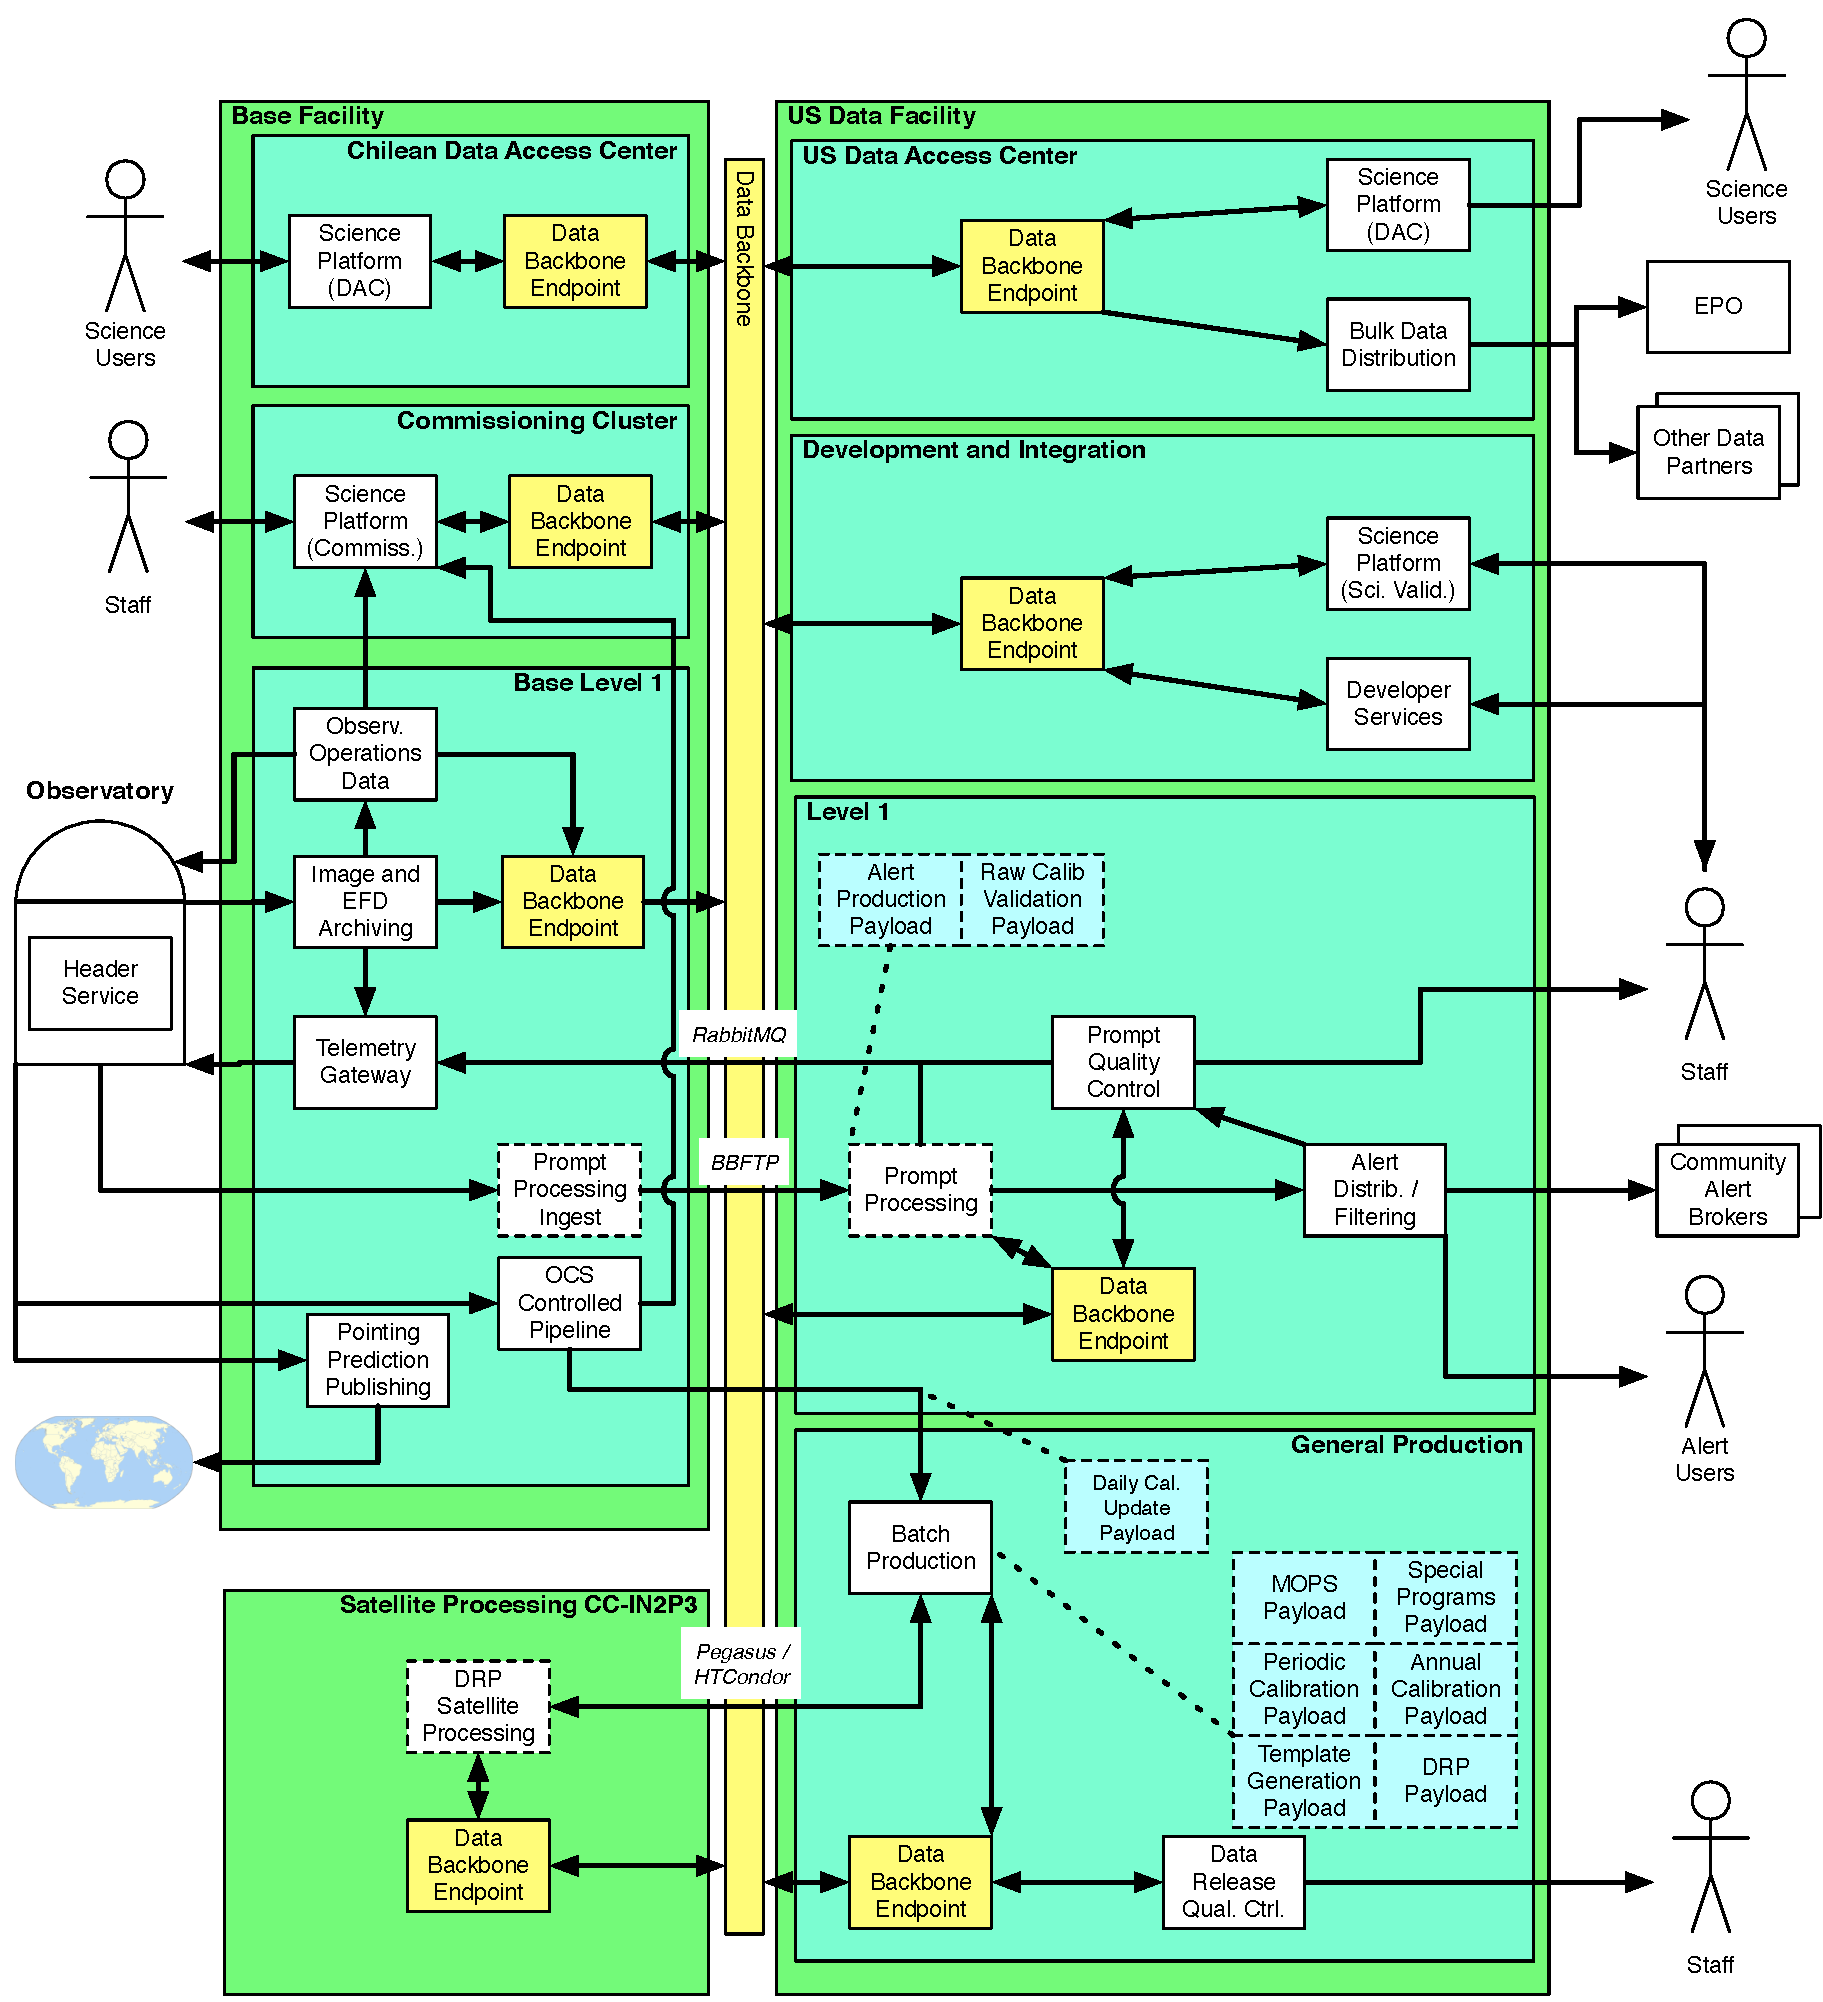
\includegraphics[width=1.0\textwidth]{images/DMS_Architecture}
	\caption{Rubin DM architecture diagram \cite{LDM-148}\label{fig:arch}}
\end{centering}
\end{figure}

\subsection{Networks} \label{sec:network}

\subsection{Data Access} \label{sec:dataaccess}

As shown in \figref{fig:vision} there are several kinds of Rubin data - mostly they are accessed via
the science platform or a community broker.
In addition some products may be accessed via and independent data access center. We will provide a few more details in this section.

\subsubsection{Data Access Centers}

\subsubsection{Alerts and Brokers}
Mention community alert brokers.
